\documentclass[aspectratio=169]{beamer}

\usepackage{graphicx}
\usepackage{amsmath}
\usepackage{xspace}
\usepackage{tikz}
\usepackage{listings}
\usepackage{unicode-math}
\usepackage{environ}
\usepackage{docs/style}
\usepackage{xepersian}

%settings---------------------
\settextfont{Yas}
\input{docs/macros}
\usetikzlibrary{arrows,calc}
\usetikzlibrary{positioning,shapes,chains,fit}


\tikzset{
    %Define style for boxes
    node/.style={
        circle,
        draw=black, thick,
        align=center,
    },
    ss/.style={
        circle,
        draw=black,
        align=center,
    },
    proc/.style={
        rounded corners,
        draw=black,
        align=center,
    },
    ifelse/.style={
	ellipse,
	draw=black,
	align=center,
    },
    cloudy/.style={
	cloud,
	cloud puffs=12,
	cloud ignores aspect,
	align=center,
	draw=black,
    },
    txt/.style={
        draw = none,
        align = center,
        font = \footnotesize,
    },
    coin/.style={
        rectangle,
        minimum height=1mm,
        minimum width=1cm,
        draw=black,
        fill=black!20,
        rounded corners
    },
    towercolor/.style={
        fill=black!80
    },
    towerbase/.style={
        trapezium,
        trapezium angle=75,
        trapezium stretches=true,
        towercolor,
        minimum width=7mm,
        minimum height=2mm,
    },
    tower/.style={
        rectangle,
        rounded corners,
        towercolor,
        minimum width=2mm,
        minimum height=26mm,
    },
    start-end/.style={
        draw,
        rectangle,
        rounded corners,
    },
    input/.style={ % requires library shapes.geometric
        draw,
        trapezium,
        trapezium left angle=60,
        trapezium right angle=120,
    },
    operation/.style={
        draw,
        rectangle
    },
    loop/.style={ % requires library shapes.misc
        draw,
        chamfered rectangle,
        chamfered rectangle xsep=2cm
    },
    decision/.style={ % requires library shapes.geometric
        draw,
        diamond,
        aspect=#1
    },
    decision/.default=1,
    print/.style={ % requires library shapes.symbols
        draw,
        tape,
        tape bend top=none
    },
    connection/.style={
        draw,
        circle,
        radius=5pt,
    },
    process rectangle outer width/.initial=0.15cm,
    predefined process/.style={
        rectangle,
        draw,
        append after command={
        \pgfextra{
          \draw
          ($(\tikzlastnode.north west)-(0,0.5\pgflinewidth)$)--
          ($(\tikzlastnode.north west)-(\pgfkeysvalueof{/tikz/process rectangle outer width},0.5\pgflinewidth)$)--
          ($(\tikzlastnode.south west)+(-\pgfkeysvalueof{/tikz/process rectangle outer width},+0.5\pgflinewidth)$)--
          ($(\tikzlastnode.south west)+(0,0.5\pgflinewidth)$);
          \draw
          ($(\tikzlastnode.north east)-(0,0.5\pgflinewidth)$)--
          ($(\tikzlastnode.north east)+(\pgfkeysvalueof{/tikz/process rectangle outer width},-0.5\pgflinewidth)$)--
          ($(\tikzlastnode.south east)+(\pgfkeysvalueof{/tikz/process rectangle outer width},0.5\pgflinewidth)$)--
          ($(\tikzlastnode.south east)+(0,0.5\pgflinewidth)$);
        }  
        },
        text width=#1,
        align=center
    },
    predefined process/.default=1.75cm,
    man op/.style={ % requires library shapes.geometric
        draw,
        trapezium,
        shape border rotate=180,
        text width=2cm,
        align=center,
    },
    extract/.style={
        draw,
        isosceles triangle,
        isosceles triangle apex angle=60,
        shape border rotate=90
    },
    merge/.style={
        draw,
        isosceles triangle,
        isosceles triangle apex angle=60,
        shape border rotate=-90
    },
}

\setmathfont{Latin Modern Math}

%cover page info--------------
\title{الگوریتم‌های پیشرفته در گراف}
\author{آرش شفیعی}
\institute{\includegraphics[height=1.2cm]{logos/ui.png}}
\date{}

\begin{document}

%cover page-------------------
\begin{frame}[plain]
	\centering{به نام خدا}
	\maketitle
\end{frame}

\setcounter{framenumber}{0}
\raggedleft

%refrences----------------
\begin{itemframe}{کتاب‌های مرجع}{}
\itmsep{5mm}
\item[-]
مقدمه‌ای بر الگوریتم‌ها از کرمن، لایسرسون، ریوست، و استاین
\fn{1}{Introduction to Algorithms, by Cormen, Leiserson, Rivest, and Stein}

\end{itemframe}

%chpaters--------------------
%------------------------------------------------------------------------
\begin{itemframe}{یادآوری}{تعریف گراف}
\item[-]
گراف‌ها به دو دسته جهت‌دار و بدون جهت تقسیم می‌شوند. این دسته بندی از این جهت مهم است که گراف‌های جهت‌دار و بدون جهت به شکل \textbf{مجزا} تعریف می‌شوند و تفاوت‌هایی در تعریف آنها وجود دارد؛
\item[۱]
گراف بدون جهت: طبق تعریف این گراف نمی‌تواند طوقه یا یال موازی داشته باشد.
\item[۲]
گراف جهت‌دار: طبق تعریف این گراف می‌تواند طوقه داشته باشد اما نمی‌تواند یال موازی داشته باشد.

\end{itemframe}
%------------------------------------------------------------------------
\begin{itemframe}{یادآوری}{تعریف گراف}
\item[-]
البته دو یال بین دو رأس یکسان در صورتی که در جهت مخالف یکدیگر باشند موازی محسوب \textbf{نمی‌شوند}. برای مثال شکل زیر یک گراف فاقد یال موازی است.
\centerimg[.2]{figs/chap01/1.png}
\item[-]
 به این یال‌ها پادموازی
\fn{1}{antiparallel}
 گفته می‌شود. بنابراین گراف جهت دار \textbf{می‌تواند} یال پادموازی داشته باشد.

\item[-]
در هر یک از مسائل بسته به ذات مسئله نوع خاصی از گراف به عنوان ورودی در نظر گرفته می‌شود. برای مثال ورودی مسئله کوتاه ترین مسیر در حالت کلی یک گراف جهت دار و وزن دار است.
\end{itemframe}

%------------------------------------------------------------------------
\begin{itemframe}{یادآوری}{تحلیل الگوریتم‌های گراف}
\item[-]
الگوریتم‌های گراف برخلاف بیشتر الگوریتم‌هایدارای دو متغییر تاثیر گذار در اندازه ورودی‌اند: تعداد یال‌ها (|E|) و تعداد رئوس (|V|) .
\item[-]
بر اساس یک قرارداد شناخته‌شده می‌توان در نمادهای مجانبی از قرار دادن نماد اندازه در اطراف V و E صرف‌نظر ‌کرد.

\item[-]
الگوریتم‌های گراف به طور معمول در دو حالت بررسی می‌شوند:
\item[الف]
زمانی که گراف متراکم باشد: در این حالت فرض میکنیم همه رئوس به هم متصل هستند بنابراین تعداد یال ها از مرتبه
\ath{V^2}
است.
\item[ب]
زمانی که گراف خلوت باشد:‌ در این حالت به طور معمول فرض می‌شود که تعداد یال‌ها از مرتبه
\ath{V}
است.
\end{itemframe}

%------------------------------------------------------------------------
\begin{itemframe}{یادآوری}{تحلیل الگوریتم‌های گراف}
\item[-]
پیچیدگی زمانی ارائه شده برای یک الگوریتم گراف را می‌توان در دو حالت بالا تحلیل کرد. برای مثال تمرین زیر را در نظر بگیرید:
\centerimg[1]{figs/chap01/2.png}

\end{itemframe}

%------------------------------------------------------------------------
\begin{itemframe}{یادآوری}{تحلیل الگوریتم‌های گراف}
\item[-]
پیچیدگی زمانی الگوریتم پریم با استفاده از هرم دودویی از مرتبه
\m{O(E logV+V lgV)}
و با استفاده از هرم فیبوناچی از مرتبه
\m{O(E+V logV)}
است. با جایگذاری V به جای E در این دو تابع درمی‌یابیم که در گراف خلوت هر دو پیاده‌سازی‌ از لحاظ مجانبی سرعت یکسانی دارند و از مرتبه
\m{O(Vlg V)}
اند. اما در گراف متراکم پیاده‌سازی با هرم فیبوناچی از لحاظ مجانبی سریع تر و از مرتبه
\m{O(lgV^2)}
 است.
\item[-]
چنین تحلیلی در دیگر الگوریتم‌‌های گراف هم کاربرد دارد. برای مثال الگوریتم فلوید-وارشال از مرتبه زمانی
\m{O(V^3)}
 است. از تحلیل این تابع می‌توان نتیجه گرفت خلوت یا متراکم بودن گراف از نظر مجانبی تاثیری بر سرعت این الگوریتم ندارد.
\end{itemframe}



 %5 pages

\begin{itemframe}{الگوریتم جانسون}
\itm
الگوریتم جانسون
\fn{Johnson Algorithm}
مانند الگوریتم فلوید وارشال برای یافتن کوتاه ترین مسیر بین هر دو راس گراف است. این الگوریتم برای گراف‌های خلوت پبچیدگی زمانی کمتری نسبت به بقیه روش‌ها (فلوید وارشال و روش شبیه‌سازی ضرب ماترسی) دارد.

\itm
الگوریتم جانسون -مانند الگوریتم بلمن فورد- می‌تواند روی گراف دارای یال منفی کوتاه ترین مسیر را به درستی محاسبه کند و وجود دور منفی در گراف را تشخیص و گزارش دهد. (گراف دارای دور منفی در مسئله کوتاه ترین مسیر یک حالت خطا محسوب می‌شود.)
%todo number of this footnote is not correct
\footnote{برای گراف دارای دور منفی یافتن کوتاه ترین مسیر ساده می‌تواند کاربرد داشته‌باشد. این مسئله ان‌پی-سخت است.}
\end{itemframe}


\begin{itemframe}{الگوریتم جانسون}
\itm
برای طراحی یک الگوریتم مسئله کوتاه‌ترین مسیر بین هر جفت رأس می‌توان V بار اجرا کردن یکی از الگوریتم‌های کوتاه‌ترین مسیرهای هم مبداء را به عنوان یک حد بالا برای مرتبه زمانی تحلیل کرد.

\itm
برای مثال
$|V|$
بار اجرای الگوریتم بلمن فورد مرتبه
$O(V^2E)$
و
$|V|$
بار اجرای الگوریتم دایجسترا مرتبه
$O(VE+V^2lgV)$
را به دست می‌دهد.
\itm
روش دوم سریع‌تر است امّا در گراف‌‌هایی که یال منفی داشته باشند به درستی کار نمی‌کند.
\end{itemframe}


\begin{itemframe}{الگوریتم جانسون}
\itm
الگوریتم جانسون نیز از ایده‌ایی مشابه استفاده می‌کند. این الگوریتم هر دو الگوریتم بلمن-فورد و دایجسترا را فراخوانی می‌کند؛
\item[۱]
جانسون در مرحله اول، الگوریتم بلمن-فورد را استفاده می‌کند تا وجود دور منفی را تشخیص دهد و در صورتی که دور منفی وجود داشت آن را گزارش داده و کار تمام می‌شود.
\item[۲]
در صورتی که دور منفی وجود نداشت، این الگوریتم با استفاده از روشی که در ادامه بررسی خواهد شد، همه وزن‌ها را به مقادیر غیر منفی نگاشت می‌کند.
\item[۳]
حال که همه وزن‌‌های غیر منفی شده‌اند برای هر رأس یک بار الگوریتم دایجسترا اجرا می‌شود تا کوتاه ترین مسیرها از هر رأس به بقیه رئوس محاسبه شوند.
\end{itemframe}


\begin{itemframe}{الگوریتم جانسون}
\itm
اما چطور باید وزن‌های گراف را به مقادیر غیر منفی نگاشت کرد؟ واضح است که بعد از تغییر وزن‌ها نباید کوتاه ترین مسیرها را تغییر کنند. برای مثال اضافه کردن یک مقدار ثابت به همه وزن‌ها نگاشت مناسبی نیست. برای درک بهتر این موضوع به مثال زیر توجه کنید:
\begin{center}
	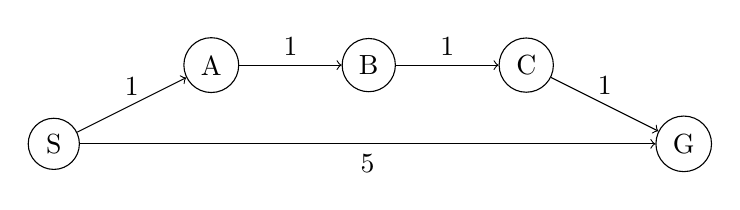
\begin{tikzpicture}[->]
		\node[circle,draw] (S) at (0,0) {S};
		\node[circle,draw] (G) at (8,0) {G};
		\node[circle,draw] (A) at (2,1) {A};
		\node[circle,draw] (B) at (4,1) {B};
		\node[circle,draw] (C) at (6,1) {C};

		\draw (S) -- node[below] {5} (G);
		\draw (S) -- node[above] {1} (A);
		\draw (A) -- node[above] {1} (B);
		\draw (B) -- node[above] {1} (C);
		\draw (C) -- node[above] {1} (G);
	\end{tikzpicture}
\end{center}
\itm
اضافه کردن یک واحد به همه یال‌ها کوتاه ترین مسیر از S به G را تغییر می‌دهد:

\begin{center}
	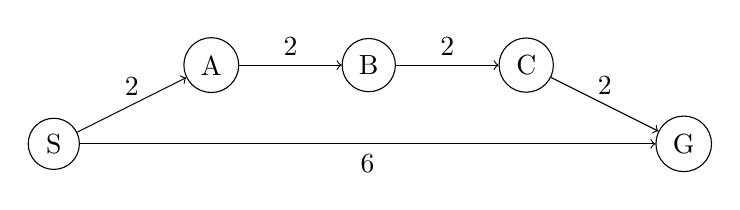
\begin{tikzpicture}[->]
		\node[circle,draw] (S) at (0,0) {S};
		\node[circle,draw] (G) at (8,0) {G};
		\node[circle,draw] (A) at (2,1) {A};
		\node[circle,draw] (B) at (4,1) {B};
		\node[circle,draw] (C) at (6,1) {C};

		\draw (S) -- node[below] {6} (G);
		\draw (S) -- node[above] {2} (A);
		\draw (A) -- node[above] {2} (B);
		\draw (B) -- node[above] {2} (C);
		\draw (C) -- node[above] {2} (G);
	\end{tikzpicture}
\end{center}
\end{itemframe}


\begin{itemframe}{الگوریتم جانسون}
\itm
بیایید ویژگی‌های این تغییر وزن را به طور دقیق‌تر بررسی کنیم؛\\
فرض کنید وزن‌های گراف توسط تابعی به نام «تابع وزن»
\fn{weight function}
داده شده. به طوری که وزن یال بین u و v برابر است با
$w(u, v)$.
آنگاه تابع وزن جدیدی مانند
$\hat{w}$
باید این دو ویژگی را داشته باشد:
\item[1]
به ازای هر
$u, v \in E$
مسیری مانند p با استفاده از تابع وزن
$w$
یک کوتاه ترین مسیر از u به v است اگر و تنها اگر مسیر p با استفاده از تابع وزن
$\hat{w}$
نیز یک کوتاه ترین مسیر باشد.
\item[2]
به ازای هر
$u, v \in E$
مقدار
$\hat{w(u, v)}$
غیر منفی باشد.
\end{itemframe}


\begin{itemframe}{الگوریتم جانسون}
\itm
الگوریتم جانسون از این تغییر وزن استفاده می‌کند:
\begin{align*}
\hat{w(u, v)} = \m{w(u, v)} + h(u) - h(v)
\end{align*}
\itm
به طوری که u رأس شروع و v رأس پایان یال است و h تابعی است که به هر رأس یک عدد حقیقی نسبت می‌دهد.
\itm
در ادامه ثابت خواهیم کرد که این تغییر وزن به ازای هر تابع h کوتاه‌ترین مسیرها را تغییر نمی‌دهد اما برای تبدیل همه وزن‌ها به مقادیر غیر منفی، تابع h باید به درستی تعریف شود.
\end{itemframe}


\begin{itemframe}{الگوریتم جانسون}
\itm
ابتدا باید ثابت ‌کنیم رابطه تغییر وزن ارائه شده ویژگی اول را ارضاء می‌کند.
\itm
فرض کنید
$ p= \langle v_0, v_1, ..., v_k \rangle$
یک مسیر از
$v_0$
به
$v_k$
باشد. همچنین وزن کل مسیر p با تابع وزن w را با  w(p) نشان می‌دهیم. آنگاه
$\hat{w}$
برابر است با:
\begin{align*}
\hat{w(p)= (\hat{w}(v_0, v_1) + h(v_0) -  h(v_1)) + (\hat{w}(v_1, v_2) + h(v_1) -  h(v_2)) + } \\
(\hat{w}(v_2, v_3) + h(v_2) -  h(v_3)) + ... + (\hat{w}(v_{k-1}, v_k) + h(v_{k-1}) -  h(v_k))
\end{align*}

\end{itemframe}


\begin{itemframe}{الگوریتم جانسون}
\itm
رابطه بالا نشان می‌دهد برای هر رأس مثل u، مقدار h(u) به وزن یک یال اضافه می‌شود و از یال بعدی کسر می‌شود (به غیر از رأس ابتدا و انتهای مسیر). بعد از ساده‌سازی به این رابطه می‌رسیم:
$$\hat{w}(p)=w(p) + h(h(v_0) - h(v_k)$$
\itm
بنابراین برای هر دو رأس مشخص به همه کوتاه‌ترین مسیرهای بین آن دو رأس یک مقدار ثابت اضافه می‌شود پس این نگاشت وزن کوتاه ترین مسیرها را تغییر نمی‌دهد.
\end{itemframe}

\begin{itemframe}{الگوریتم جانسون}
\itm
هدف بعدی این است که شرایطی فراهم کنیم که ویژگی دوم هم برقرار باشد. برای این کار یک رأس جدید به نام s به گراف اضافه می‌کنیم. سپس این رأس را با یال‌هایی با وزن صفر به همه رئوس دیگر متصل می‌کنیم به طوری که یال ‌ها از s خارج شوند.
\centerimg[.4]{figs/shortest-path/4.png}
شکل بالا نمونه‌ایی از این تغییر را نشان می‌دهد (رأس آبی رنگ به گراف اضافه شده‌است).
\end{itemframe}


\begin{itemframe}{الگوریتم جانسون}
\itm
سپس تعریف می‌کنیم مقدار h برای هر رأس مثل v برابر است با کوتاه ترین مسیر از s به v . در شکل بالا نیز اعداد نوشته‌شده بر رأس‌ها به همین طریق محاسبه شده‌اند.
\itm
حال با استفاده از نامساوی مثلثاتی می‌دانیم که به ازای هر

$(u, v \in E)$
رابطه زیر برقرار است:
$$
h(v) \leqslant h(u)+w(u, v)
$$
\itm
اگر رابطه بالا برقرار نباشد نتیجه می‌شود که مسیر h(v) کوتاه‌ترین مسیر نبوده و به تناقض می‌رسیم.
\itm
سپس h(u) را به سمت راست نامساوی می‌بریم:
$$
0\leqslant w(u, v) + h(u) - h(v)
$$
\itm
سمت راست این نامساوی همان رابطه‌ایی است که برای $\hat{w}$ تعریف شد. بنابراین ثابت شد که به ازای هر
$(u, v \in E)$
مقدار $\hat{w}$ غیر منفی است.
\end{itemframe}


\begin{itemframe}{الگوریتم جانسون}
\itm
درستی الگوریتم جانسون ثابت شد. شکل زیر یک نمونه از گراف تغییر وزن یافته توسط الگوریتم جانسون است:
\centerimg[.3]{figs/shortest-path/5.png}

\itm
قبلا اشاره شد که الگوریتم جانسون از الگوریتم بلمن-فورد برای تشخیص دور منفی استفاده می‌کند. همچنین دیدم که برای محاسبه تابع h نیاز به مقادیر کوتاه‌ترین مسیر از s به بقیه رئوس نیاز داریم. می‌دانیم الگوریتم بلمن-فورد توانایی محاسبه هر دوی این موارد را دارد. بنابراین الگوریتم جانسون با یک بار اجرای بلمن-فورد هم کوتاه‌ترین مسیرها از s را محاسبه می‌کند و هم وجود دور منفی را تشخیص می‌دهد.
\end{itemframe}


\begin{itemframe}{الگوریتم جانسون}
\itm
برای یافتن وزن اصلی یک مسیر از رابطه زیر استفاده می‌کنیم:
$$
w(p(u, v)) = \hat{w}(p(u, v)) + h(v) - h(u)
$$
\itm
در نهایت به تحیلی پیچیدگی زمانی الگوریتم جانسون می‌پردازیم:
\itm
اجرای $|V|$ بار الگوریتم دایجسترا زمان‌برترین مرحله الگوریتم جانسون است بنابراین -مانند دایجسترا- باید گراف را در لیست مجاورتی ذخیره کنیم. حال اگر فرض کنیم الگوریتم دایجسترا با استفاده از هرم فیبوناچی پیاده‌سازی شده‌است، پیچیدگی زمانی برابر است با
$O(V^2lgV+VE)$
که از ضرب یک
$|V|$
در مرتبه زمانی دایجسترا به دست آمده‌است.
\itm
در صورتی که گراف خلوت باشد مرتبه زمانی این الگوریتم برابر است
$O(V^2lgV)$.
در حالی که الگوریتم فلوید-وارشال برای گراف خلوت از مربته زمانی
$O(V^3)$
است.
\end{itemframe} %12 pages
%------------------------------------------------------------------------
\begin{itemframe}{مسئله شار بیشینه}{معرفی مسئله}
\item [-]
در دنیای واقعی شبکه‌های بسیاری وجود دارند که با هدف انتقال چیزی ساخته شده‌اند. برای مثال شبکه‌های آب رسانی، مدارات الکتریکی(انتقال جریان الکتریکی)، خطوط راه‌آهن و غیره. به طور معمول در چنین شبکه‌هایی افزایش نرخ انتقال مطلوب است. بنابراین مسئله شار بیشینه می‌پرسد‌: چگونه می‌توان نرخ انتقال را در این شبکه‌ها بیشینه کرد؟
\item [-]
برای حل یک مسئله شار بیشینه باید شبکه را توسط گراف مدلسازی کرد. به این گراف «شبکه شار»
\fn{1}{flow network}
و به هر چیزی که در این شبکه در جریان باشد به طور کلی شار
\fn{2}{flow}
 گفته می‌شود.
\end{itemframe}

%------------------------------------------------------------------------
\begin{itemframe}{مسئله شار بیشینه}{معرفی مسئله}
	\item [-]
برای درک بهتر مسئله شار بییشیه ويژگی‌های این مسئله را همراه با مثال شبکه آب رسانی توضیح می‌دهیم؛
	\item
در مسئله شار بیشیه گراف ثابت فرض می‌شود. (مثال: خطوط آب‌رسانی مثل لوله‌ها و اتصالات از قبل ساخته شده‌ و غیر قابل تغییر اند.)
	\item
هر یال یک ظرفیت مشخص برای انتقال شار دارد و نمی‌تواند بیشتر از آن مقدار انتقال دهد. (مثال: هر لوله آب -بسته به قطر لوله‌- می‌تواند مقدار آبی مشخصی را از خود عبور دهد.)
	\item
سرعت انتقال شار در سراسر شبکه ثابت فرض می‌شود. (مثال: نمی‌توانیم تعیین کنیم آب با فشار بیشتری وارد لوله‌ها شود بنابراین سرعت حرکت آب در لوله‌ها یکسان است.)
\end{itemframe}

%------------------------------------------------------------------------
\begin{itemframe}{مسئله شار بیشینه}{معرفی مسئله}

	\item
در مسئله شار بیشینه تنها متغییری که ما می‌توانیم تعیین کنیم این است که چقدر از ظرفیت هر یال برای انتقال شار استفاده کنیم. (مثال: می‌توانیم یک شیر آب سر راه هر لوله قرار دهیم و بعد از حل مسئله شار بیشینه تعیین کنیم هر شیر اجازه ورود چه حجمی از آب را بدهد.)
	\item
مجموع شار ورودی به هر رأس باید با مجموع شار خروجی برابر باشد. به عبارت دیگر هیچ شاری نمی‌تواند در رأس‌های گراف ذخیره شود یا از بین برود. به این قانون، قانون بقای شار
\fn{1}{flow conservation}
گفته می‌شود.
(مثال: بدیهیست در اتصالاتی که لوله‌ها را به هم وصل می‌کند آب نمی‌تواند ذخیره شود یا نشت کند. ممکن هر اتصال یک یا چند لوله ورودی و خروجی داشته باشد در هر صورت مجموع آب ورودی و خروجی باید برابر باشد.)

\end{itemframe}

%------------------------------------------------------------------------
\begin{itemframe}{مسئله شار بیشینه}{معرفی مسئله}

	\item[-]
با این توضیحات شاید به نظر برسد که برای حل این مسئله کافیست به طور حریصانه از همه ظرفیت همه یال‌ها برای انتقال استفاده کنیم. (مثال: همه شیر آب‌هایی که سر راه لوله‌ها قرار گرفته اند را تا بیشترین مقدار باز کنیم تا در صورتی که مقدار کافی آب به آن لوله رسید از تمام ظرفیت آن لوله برای انتقال آب استفاده کنیم.)
	\item[-]
نکته جالب اینجاست که برخلاف انتظار این الگوریتم حریصانه جواب بهنیه را تولید نمی‌کند. در ادامه مثال‌هایی خواهیم دید که ممکن است کاهش مقدار شار گذرنده از یک یال باعث افزایش شار کلی گذرنده از شبکه شود. (مثال: در شبکه آب رسانی ممکن است با بستن شیر، اجازه ورود حجم کمتری از آب به یک لوله را بدهیم و با این کار شار گذرنده از شبکه را بیشتر کنیم.)
\end{itemframe}

%------------------------------------------------------------------------
\begin{itemframe}{مسئله شار بیشینه}{تعاریف رسمی}
\item[-]
قبل ادامه بحث بهتر است با یک تعریف دقیق و رسمی از شبکه شار آشنا شویم؛
\item
شبکه شار یک گراف جهت‌دار است. به این معنی که شار نمی‌تواند در یک یال در دو جهت حرکت کند.

شبکه شار همرا با تابع c به ورودی مسئله داده می‌شود. تابع c یال‌ها و ظرفیت‌‌ها را نگاشت می‌کند به طوری که ظرفیت یال u به v برابر است با
\m{c(u, v)} .
\item
شبکه شار دارای در رأس خاص است که ورود شار به شبکه (و یا تولید شار) و خروج از شار شبکه (و یا مصرف شار) را مدل می‌کنند. به این دو رأس منبع
\fn{1}{source}
و مقصد
\fn{2}{sink}
گفته می‌شود. به طور معمول به رأس منبع با s و رأس مقصد با t نشان داده می‌شوند.
\item
رأس منبع و مقصد تنها رئوسی هستند که از قانون بقای شار پیروی نمیکنند.
\end{itemframe}

%------------------------------------------------------------------------
\begin{itemframe}{مسئله شار بیشینه}{تعاریف رسمی}
\item[-]
همانطور که قبلا اشاره شد، گراف جهت‌دار می‌تواند طوقه داشته‌باشد. امّا وجود طوقه در شبکه شار غیر مجاز است.
\item[-]
همچنین دیدیم که وجود یال‌های پادموازی نیز در گراف جهت‌دار بلامانع است. امّا در شبکه شار یال‌های پادموازی هم غیر مجاز اند.(در بخش يادآوری فصل یال‌های پادموازی بحث شده‌اند.)
\item[-]
حذف طوقه (دور به طول ۱) و یال‌های پادموازی (دور به طول ۲) از پیچیدگی مسئله می‌کاهد.
\item[-]
وجود دورهایی با طول بالا تر در شبکه شار مجاز است.
\end{itemframe}

%------------------------------------------------------------------------
\begin{itemframe}{مسئله شار بیشینه}{تعاریف رسمی}

\item[-]
همچنین باید یک تعریف کمی برای شار کل شبکه ارائه کنیم تا مشخص شود منظور از شار بیشینه چیست؛
\item
خروجی این مسئله کردن تابع f است که یال‌ها را به شار گذرنده از آنها نگاشت می‌کند. به این صورت که شار گذرنده از یال u به v برابر است با
\m{f(u, v)} .

\item
مقدار شار کل شبکه با |f| نشان داده می‌شود و به این صورت تعریف می‌شود: \\
\begin{center}
\m{|f| = \sum_{v \in V} f(s, v) - \sum_{v \in V} f(v, s)}
\end{center}
\item
به زبان ساده این عبارت مجموع شار خالص خروجی از رأس منبع را مشخص می‌کند :مجموع شار خارج شونده از منبع منهای مجموع شار وارد شونده به منبع. (معولا مجموع شار وارد شونده به منبع صفر است.)
\end{itemframe}
%------------------------------------------------------------------------
\begin{itemframe}{مسئله شار بیشینه}{تعاریف رسمی}
\item[-]
امّا چطور این کمیّت می‌تواند نماینده شار گذرنده از کل شبکه باشد؟
\item
برای درک بهتر این موضوع به شبکه شار به چشم یک بلوک بزرگ نگاه کنید که از رأس منبع شار به آن وارد و از مقصد خارج می‌شود.
\centerimg[.5]{figs/chap01/6.png}

\item
با توجه به قانون بقای شار، شار نمی‌تواند در این بلوک بزرگ بماند بنابراین با همان نرخی که وارد آن می‌شود باید از آن خارج شود. (فرض کنید پیکان‌ها شار خالص را نشان می‌دهند.)‌
\item
بنابراین نرخ خالص شار خروجی از منبع نماینده شاری است که در کل شبکه جریان دارد.
\end{itemframe}


%------------------------------------------------------------------------
\begin{itemframe}{مسئله شار بیشینه}{ساده‌سازی مسئله شار بیشینه}
\item[-]
شاید دقت کرده باشید که در تعریف شبکه شار فرض‌های ساده کننده‌ایی درنظر گرفتیم که لزوماً در یک مسئله واقعی بیشینه‌سازی شار، برقرار نیستند. دو فرض به این شکل داشتیم که در زیر آورده شده‌اند؛
\item[۱]
ممکن است در یک مسئله واقعی بیشینه‌سازی شار چند منبع و چند مقصد داشته باشیم. در حالی که در تعریف شبکه شار تنها یک منبع و مقصد برای شبکه لحاظ کردیم.
\item[۲]
ممکن است در یک مسئله واقعی بیشینه‌سازی شار یال موازی داشته باشیم. درحالی که وجود چنین یالی را در شبکه شار غیر مجاز دانستیم.
\end{itemframe}

%------------------------------------------------------------------------
\begin{itemframe}{مسئله شار بیشینه}{ساده‌سازی مسئله شار بیشینه}
\item[-]
در ادامه نشان می‌دهیم که چطور یک مسئله واقعی بیشینه‌سازی شار را که دارای چند منبع و مقصد است و یال پادمتقارن دارد را مدل کنیم.

\end{itemframe}

%------------------------------------------------------------------------
\begin{itemframe}{مسئله شار بیشینه}{ساده‌سازی مسئله شار بیشینه}
\item
شکل زیر نشان می‌دهد چطور یک شبکه شار با چندین رأس منبع و مقصد را می‌توان به یک شبکه شار با یک منبع و مقصد تبدیل کرد.
\centerimg[.8]{figs/chap01/7.png}

\end{itemframe}

%------------------------------------------------------------------------
\begin{itemframe}{مسئله شار بیشینه}{ساده‌سازی مسئله شار بیشینه}
\item
شکل زیر نشان می‌دهد چطور یک شبکه دارای یال‌های پادمتقارن را می‌توان به یک شبکه شار قابل‌قبول تبدیل کرد.
\centerimg[.9]{figs/chap01/8.png}
\end{itemframe} %16 pages
%------------------------------------------------------------------------
\begin{itemframe}{مسئله شار بیشینه}{روش فورد-فولکرسون}
\item[-]
روش فورد-فولکرسون
\fn{1}{Ford-Fulkerson method}
برای حل مسئله شار بیشینه طراحی شده‌است. بهتر است که به فورد-فولکرسون «الگوریتم» گفته نشود زیرا پیاده‌سازی دقیقی را مشخص نمی‌کند. بلکه یک چارچوب کلی برای حل مسئله شار بیشینه ارائه می‌دهد و چند پیاده‌سازی مختلف با زمان‌های اجرای متفاوت دارد.
\item[-]
\end{itemframe}


%------------------------------------------------------------------------
\begin{itemframe}{مسئله شار بیشینه}{اثبات روش فورد-فولکرسون}
\item[-]
با نحوه کار روش فورد-فولکرسون آشنا شدیم. امّا چرا این روش به درستی کار می‌کند؟
\item[-]
در این بخش اثبات درستی این روش را خواهیم دید. برای اثبات‌ها نیاز است مفاهیمی که در بخش قبل با آنها آشنا شدیم را به طور رسمی به زبان ریاضی تعریف کنیم.
\end{itemframe}

%------------------------------------------------------------------------
\begin{itemframe}{مسئله شار بیشینه}{اثبات روش فورد-فولکرسون}
\item[-]
تعریف رسمی گراف متمم:
\item
در تعریف شبکه شار گفتیم f تابعیست که شار یال‌ها را بازمی‌گرداند. برای شبکه شار G با تابع ظرفیت c و یک شار مانند f بر روی این شبکه، گراف متمم را با
\m{G_f}
و شار آن را با
\m{f'}
 نشان می‌دهیم.
\item
 دقت کنید که f جزئی از تعریف G نیست و یک شبکه شار می‌تواند f های مختلفی داشته باشد. بنابراین این نحوه نوشتار (
\m{G_f}
) مشخص می‌کند گراف متمم متناظر با کدام شبکه و کدام شار از شبکه است.
\end{itemframe}

%------------------------------------------------------------------------
\begin{itemframe}{مسئله شار بیشینه}{اثبات روش فورد-فولکرسون}
\item
تابع ظرفیت گراف متمم به این صورت تعریف می‌شود:
\begin{align}
c_f(u, v)=
\begin{cases}
c(u, v) - f(u, v) & \text{if } (u, v) \in E\\
f(v, u) & \text{if } (v, u) \in E\\
0 & \text{otherwise}
\end{cases}
\label{res-net-cap}
\end{align}

\item
تعریف می‌کنیم مقدار تابع c برای یال‌هایی که در گراف وجود ندارند صفر است(پیش از این اشاره کردیم که تابع f نیز همین ویژگی را دارد). این مسئله برای فهم فرمول بالا ضروری است. برای درک بهتر فرمول بالا را در حالت‌های حدی بررسی کنید.(از ظرفیت یال کاملاً استفاده شود، شار یک یال دارای ظرفیت صفر باشد، بین دو رأس یالی وجود نداشته باشد)

\end{itemframe}

%------------------------------------------------------------------------
\begin{itemframe}{مسئله شار بیشینه}{اثبات روش فورد-فولکرسون}
\item[-]
تعریف افزایش شار:
\item
به اعمال تغییرات گراف متمم بر شبکه شار augmentation گفته می‌شود. در ترجمه فارسی از کلمه «افزایش» استفاده می‌کنیم هرچند منظور از این ترجمه، افزایش شار نیست بلکه افزودن شار گراف متمم بر شارِ شبکه شار است.
\item
افزودن شار f به
\m{f'}
را با
\m{f \uparrow f'}
نشان می‌دهیم. و به این صورت تعریف میکنیم:
\begin{align}
f \uparrow f'(u, v)=
\begin{cases}
f(u, v)+f'(u, v)-f'(v, u)& \text{if} (u, v) \in E\\
0 &\text{otherwise}
\end{cases}
\label{aug-flow-def}
\end{align}
\end{itemframe}

%------------------------------------------------------------------------
\begin{itemframe}{مسئله شار بیشینه}{اثبات روش فورد-فولکرسون}
\item[-]
\m{f \uparrow f'}
نیز یک تابع است که به هر جفت رأس یک مقدار نسبت می‌دهد. ادعا می‌کنیم که این تابع نیز تابع شار است و می‌توانیم آن را جایگزین f کنیم. برای اثبات این ادعا باید ثابت کنیم
\m{f \uparrow f'}
ویژگی‌های تابع شار را دارد. تابع شار تابعی است که به هر جفت رأس یک مقدار نسبت می‌دهد و:
\item[1]
از ظرفیت‌های شبکه شار تجاوز نمی‌کند.
\item[2]
از قانون پایستگی شار پیروی می‌کند.
\item
بنابراین باید بررسی آیا
\m{f \uparrow f'}
این دو ویژگی را دارد یا خیر.
\end{itemframe}

%------------------------------------------------------------------------
\begin{itemframe}{مسئله شار بیشینه}{اثبات روش فورد-فولکرسون}
\item[-]
ویژگی اول به سادگی با توجه به فرمول‌های ۱ و ۲ اثبات می‌شوند. به فرمول ۱ دقت کنید‍؛ شار ظرفیت موافق به دقیقا برابر با تفاضل شار فعلی و حداکثر ظرفیت تعریف می‌شود بنابراین حتی اگر از تمام ظرفیت یال موافق در گراف متمم استفاده کنیم، شار
\m{f \uparrow f'}
از حداکثر نفوذ نمی‌کند.
\item
به دلایل مشابه و با توجه به تعاریف می‌توان اثبات کرد که شار
\m{f \uparrow f'}
از صفر کمتر نمی‌شود.
\end{itemframe}
%------------------------------------------------------------------------
\begin{itemframe}{مسئله شار بیشینه}{اثبات روش فورد-فولکرسون}
\item[-]
برای اثبات ویژگی دوم (پایستگی شار) ابتدا باید ثابت کنیم این رابطه برای هر u برقرار است:

\begin{align}
\sum_{v\in V} f \uparrow f'(u, v)  & - \sum_{v\in V} f \uparrow f'(v, u) \notag \\
&=
 \sum_{v\in V} f(u, v) - \sum_{v\in V} f (v, u)
+
\sum_{v\in V} f'(u, v) - \sum_{v\in V} f'(v, u)
\label{cons}
\end{align}
\item

به زبان ساده این رابطه می‌گوید به ازای هر رأس مثل u\\
تفاضل شار وارد و خارج شونده به u در
\m{ f \uparrow f'} \\
=\\
تفاضل شار وارد و خارج شونده به u در
\m{f} \\
+\\
تفاضل شار وارد و خارج شونده به u در
\m{f'}\\


\end{itemframe}
%------------------------------------------------------------------------
\begin{itemframe}{مسئله شار بیشینه}{اثبات روش فورد-فولکرسون}
\item
در اینجا تساوی \ref{cons} را اثبات نمی‌کنیم. با اعمال رابطه \ref{aug-flow-def} به سمت چپ تساوی این اثبات قابل انجام است. امّا درستی این رابطه به صورت شهودی نیز قابل فهم است؛
\\
شار گراف متمم به همه یال‌ها افزوده شده بنابراین انتظار داریم مقدار شار ورودی به هر رأس، به اندازه شار ورودی به همان رأس در
\m{f'}
افزایش داشته‌باشد. این مسئله برای مجموع شار خروجی نیز صادق است.
\item
به
\eq{cons}
دقت کنید. سمت راست این تساوی برابر صفر است زیرا پایستگی در هر دو شار
\m{f}
و
\m{f'}
برقرار است. بنابراین در هر دو، شار وارد شونده به یک رأس با شار خارج شونده از آن برابر است. (به غیر از s و t که پایستگی شار در آنها وجود ندارد.)
\end{itemframe}
%------------------------------------------------------------------------
\begin{itemframe}{مسئله شار بیشینه}{اثبات روش فورد-فولکرسون}
\item
حال اگر سمت راست \eq{cons} را صفر بگذاریم نتیجه می‌گیریم:
\begin{align*}
\sum_{v\in V} f \uparrow f'(u, v)  = \sum_{v\in V} f \uparrow f'(v, u)
\end{align*}

\item
بنابراین پایستگی شار در
\m{ f \uparrow f'}
برقرار است. توجه کنید که
\m{f}
و
\m{f'}
هر دو قانون پایستگی شار را رعایت می‌کنند بنابراین قابل انتظار است که شار حاصل افزودن این دو شار نیز چنین باشد.
\end{itemframe}
%------------------------------------------------------------------------
\begin{itemframe}{مسئله شار بیشینه}{اثبات روش فورد-فولکرسون}
\item [-]
تا اینجا ثابت کردیم
\m{ f \uparrow f'}
یک تابع شار است پس قابلیت اعمال بر شبکه شار را دارد، امّا این کافی نیست. می‌خواهیم انجام این کار باعث افزایش مقدار
\m{|f|}
شود. به عبارت دیگر
\m{|f \uparrow f'|}
بزرگ‌تر از
\m{|f|}
باشد.
\item
خواهیم دید که اگر
\m{f'}
به این صورت تعریف شود، این اتفاق همیشه می‌افتد:
\begin{align}
f_p(u, v)=
\begin{cases}
c_p& \text{if} (u, v) \in P\\
0 &\text{otherwise}
\end{cases}
\label{aug-path}
\end{align}


\item
در تعریف بالا p یک مسیر افزایشی در گراف متمم است. و
\m{c_p}
بیشترین شاری است که می‌تواند در این مسیر جریان یابد. این مقدار برابر است با:
\begin{align}
c_f(p) = min \{c_f(u, v): (u, v) \in p\}
\label{path-cap}
\end{align}

\end{itemframe}
%------------------------------------------------------------------------

\begin{itemframe}{مسئله شار بیشینه}{اثبات روش فورد-فولکرسون}

\item
برای اینکه ثابت کنیم افزودن
\m{f_p}
به
\m{f}
مقدار
\m{|f|}
را افزایش می‌دهد. باید ثابت کنیم این رابطه برقرار است:
\begin{align}
|f \uparrow f'|=|f| + |f'|
\label{aug-flow-sum}
\end{align}
\item

پیش از این با
\eq{cons}
آشنا شدیم. دیدیم این معادله به ازای هر
\m{u \in E}
برقرار است. کافیست به جای u رأس s را در آن قرار دهید تا
\eq{aug-flow-sum}
نتیجه شود. (توجه کنید که در دو رأس s و t پایستگی شار وجود ندارد بنابراین سمت راست تساوی لزوماُ برابر صفر نخواهد‌شد.)
\item
به زبان ساده این رابطه می‌گوید مقدار شار در شبکه شار افزایش یافته (augmented) برابر است با مجوع شار شبکه شار اولیه و گراف متمم.
\end{itemframe}
%------------------------------------------------------------------------

\begin{itemframe}{مسئله شار بیشینه}{اثبات روش فورد-فولکرسون}
\item
بنابراین طبق
\eq{aug-flow-sum}
می‌دانیم:
\begin{align*}
|f \uparrow f_p| = |f| + |f_p|
\end{align*}
\item
کافیست ثابت کنیم شار گراف متمم که از روی یک مسیر افزایشی به دست آمده الزاماً مثبت است و بنابراین
\begin{align*}
|f \uparrow f_p| > |f|
\end{align*}
\item
اثبات اینکه
\m{|f_p|}
مثبت است ساده است؛ می‌دانیم p یک مسیر ساده از s به t است بنابراین نمی‌تواند یال ورودی به s داشته باشد و دقیقا یک یال خروجی از s دارد.
\item
شار گذرنده از یال خروجی s برابر با کمترین ظرفیت مسیر p است(
\eq{path-cap}
).  می‌دانیم یالی در مسیر p وجود ندارد که ظرفیت ۰ یا منفی داشته باشد. زیرا چنین یالی اصلاً در گراف متمم وجود ندارد (طبق تعریف، ظرفیت مقداری مثبت است و ظرفیت صفر به معنای عدم وجود یال در گراف متمم است.)
\end{itemframe}

%------------------------------------------------------------------------
\begin{itemframe}{مسئله شار بیشینه}{اثبات روش فورد-فولکرسون}
\item[-]
تا اینجا دیدیم برای افزایش شار کافیست یک مسیر افزایشی در گراف متمم پیدا کنیم و با استفاده از آن عملیات افزایش را روی شبکه شار انجام دهیم و سپس دوباره همین عمل را انجام دهیم. امّا شرط خاتمه چیست؟ چطور می‌توانیم از بهنیه بودن جواب اطمینان یابیم؟
\item[-]
قضیه «شار بیشینه، برش کمینه»
\fn{1}{Max-fow min-cut theorem}
به این سوال اینگونه پاسخ می‌دهد:

درصورتی که هیچ مسیر افزایشی در گراف متمم وجود نداشته باشد شار موجود در شبکه شار بیشینه است.
\end{itemframe}

%------------------------------------------------------------------------
\begin{itemframe}{مسئله شار بیشینه}{اثبات روش فورد-فولکرسون}
\item[-]
به طور دقیق‌تر قضیه «شار بیشینه، برش کمینه» بیان می‌کند این سه گزاره هم ارز هستند:
\item[1]
f یک شار بیشینه در G باشد.
\item[2]
گراف متمم \m{G_f} مسیر افزایشی نداشته باشد.
\item[3]
مقدار شار برابر با ظرفیت یک برش از گراف باشد.
\item[-]
برش و ظرفیت برش را در ادامه تعریف خواهیم کرد.
\end{itemframe}
%------------------------------------------------------------------------
\begin{itemframe}{مسئله شار بیشینه}{اثبات روش فورد-فولکرسون}
\item[-]
هم ارز بودن گزاره‌های اول و دوم برای اطمینان از صحت الگوریتم کفایت می‌کند امّا برای اثبات این قضیه این مسیر را طی می‌کنیم:
\begin{align*}
\{(1 \Rightarrow 2) \land (2 \Rightarrow 3) \land (3 \Rightarrow 1)\}
\Rightarrow
\{1 \Leftrightarrow 2 \Leftrightarrow 3 \}
\end{align*}
\item[-]
بنابراین گزاره سوم در اثبات کمک می‌کند. به اینکه چگونه از سه عبارت سمت چپ هم ارزی دو گزاره را ثابت کردیم دقت کنید. مثلاً برای اثبات هم‌ارزی ۳ و ۱ کافیست یک بار از ۳ شروع کنید و ۱ را نتیجه بگیرید و بار دیگر از ۳ شروع و ۱ را نتیجه بگیرید:
\begin{align*}
\{(1 \Rightarrow 2) \land (2 \Rightarrow 3)\}
\land
\{(3 \Rightarrow 1)\}
\Rightarrow
\{(3 \Leftrightarrow 1)\}
\end{align*}

\end{itemframe}

%------------------------------------------------------------------------
\begin{itemframe}{مسئله شار بیشینه}{اثبات روش فورد-فولکرسون}
\item[-]
بنابراین برای اثبات این قضیه باید با برش
\fn{1}{cut}
 و ویژگی‌های آن بیشتر آشنا شویم. ممکن است این مفهوم را در بحث درخت پوشای کمینه دیده باشید. یک برش گراف را به دو مجموعه رأس S و T تقسیم می‌کند. برش در شبکه شار نیز شبیه به گراف معمولی است با این تفاوت که رأس منبع باید در S و رأس مقصد در T‌ باشد. بنابراین هر دو نمی‌توانند در یک بخش باشند.
\item[-]
کمیتی به نام ظرفیت برش برابر است با کل ظرفیت یال‌هایی که شروع آنها از S است و پایان آنها در T باشد:
\begin{align*}
c(S, T) = \sum_{u \in S}  \sum_{v \in T} c(u, v)
\end{align*}

\end{itemframe}

%------------------------------------------------------------------------
\begin{itemframe}{مسئله شار بیشینه}{اثبات روش فورد-فولکرسون}
\item[-]
همچنین شار خالصی
\fn{1}{net flow}
 که از S به سمت T در جریان است را با
\m{f(S, T)}
نشان داده و به این صورت تعریف می‌کنیم:
\begin{align}
f(S, T) = \sum_{u \in S}  \sum_{v \in T} f(u, v)  - \sum_{u \in S}  \sum_{v \in T} f(v, u)
\label{cut-net-flow}
\end{align}
\item[-]
شار خالص ترجمه عبارت net flow است. این عبارت برای کمیتی به کار می‌رود که حاصل کسر شارهای جهت مخالف از شارهای موافق باشد. برای مثال \eq{cut-net-flow} شار خالص گذرنده از یک برش را نشان می‌دهد.
\end{itemframe}

%------------------------------------------------------------------------
\begin{itemframe}{مسئله شار بیشینه}{اثبات روش فورد-فولکرسون}
\item[-]
به برشی که کمترین ظرفیت را در میان تمام برش‌ها داشته باشد «برش کمینه»
\fn{1}{minimum cut}
 گفته می‌شود.
\item[-]
برش در شبکه شار ویژگی مهمی دارد که در اثبات قضیه شار بیشینه، برش کمینه به ما کمک می‌کند. به این صورت که شار خالص گذرنده از هر برش دلخواه (که در \eq{cut-net-flow} تعریف کردیم) با |f| برابر است.

\item[-]
از این ویژگی می‌توان نتیجه گرفت مقدار شار نمی‌تواند از ظرفیت برش کمینه بیشتر باشد. اگر فرض کنیم |f| بیشتر از ظرفیت یک برش باشد به تناقض می‌رسیم. زیرا می‌دانیم شار خالص این برش |f| در  حالی که ظرفیت این برش از |f| کمتر است.
\item[-]
بنابراین ظرفیت هر برش یک حد بالا برای |f| است.
\end{itemframe}

%------------------------------------------------------------------------
\begin{itemframe}{مسئله شار بیشینه}{اثبات روش فورد-فولکرسون}
\item[-]
حال که با برش در شبکه شار آشنا شدیم می‌توانیم قضیه «شار بیشینه برش کمینه» را ثابت کنیم. طبق مسیر کلی‌ایی که پیش از این ارائه شد، ابتدا باید ثابت کنیم در صورتی که مقدار شار بیشینه باشد در گراف متمم مسیر افزایشی وجود ندارد (\m{1 \Rightarrow 2}).
\item[-]
فرض کنید f شار بیشینه است و یک مسیر افزایشی مانند p در گراف متمم وجود دارد. پیش از این دیدیم که افزودن شار مسیر افزایشی به شار فعلی باعث افزایش |f| می‌شود. بنابراین  \m{|f \uparrow f_p|} از \m{|f| } بیشتر است که این با فرض اولیه در تناقض است. بنابراین در صورتی که شار بیشینه باشد مسیر افزایشی نمی‌تواند در گراف متمم وجود داشته باشد.
\end{itemframe}
%------------------------------------------------------------------------
\begin{itemframe}{مسئله شار بیشینه}{اثبات روش فورد-فولکرسون}
\item[-]
دٰر قدم بعد باید ثابت کنیم اگر گراف متمم شامل مسیر افزایشی نباشد، مقدار شار با ظرفیت یکی از برش‌ها برابر است. (\m{2 \Rightarrow 3}).
\item[-]
فرض کنیم گراف متمم مسیر افزایشی نداشته باشد. می‌خواهیم برشی بیابیم که شار خالص آن  ظرفیت آن برابر باشد. همچنین می‌دانیم شار خالص هر برش نیز با |f| برابر است.
\item[-]
مجموعه S را تمام رأس‌هایی تعریف می‌کنم که در \textbf{گراف متمم} از رأس منبع به آنها مسیر وجود دارد و بقیه رأس‌ها در مجموعه V قرار می‌گیرند. طبق تعریف ( \eq{cut-net-flow} ) شار خالص این برش برابر است با:
\begin{align*}
f(S, T) = \sum_{u \in S} \sum_{v \in T} f(u, v) - \sum_{v \in T} \sum_{u \in S} f(v, u)
\end{align*}
\end{itemframe}
%------------------------------------------------------------------------
\begin{itemframe}{مسئله شار بیشینه}{اثبات روش فورد-فولکرسون}
\item[-]
به عبارت زیر که قسمتی از معادله بالاست دقت کنید:
\begin{align*}
\sum_{u \in S} \sum_{v \in T} f(u, v)
\end{align*}
یادآوری می‌شود که تابع شار برای یال‌هایی که وجود ندارند صفر است. بنابراین در عمل این عبارت مجموع یال‌هایی است که بین دو بخش گراف وجود دارند و جهت آنها از S به T است. ادعا می‌کنیم که شار گذرنده از همه این یال‌ها برابر با ظرفیت آنهاست.
\item[-]
برای اثبات این ادعا فرض کنید شار یک یال از
\m{x \in S}
به
\m{y \in T}
از ظرفیت آن کمتر باشد بنابراین یک یال از x به y باید در گراف متمم وجود داشته باشد که نشان دهنده امکان افزایش شار است (طبق \eq{res-net-cap}). می‌دانیم از s به x مسیر وجود دارد زیرا این رأس در مجموعه S است. اگر x به y مسیر داشته باشد پس از s به y هم یک مسیر وجود دارد امّا y در مجموعه S نیست و اینجا به تناقض می‌رسیم.

\end{itemframe}
%------------------------------------------------------------------------
\begin{itemframe}{مسئله شار بیشینه}{اثبات روش فورد-فولکرسون}
\item[-]
با استدلال مشابه می‌توانیم ثابت کنیم که قسمت دوم عبارت برابر صفر است. این عبارت نیز مجموع ظرفیت همان یال‌های بین دو بخش است با این تفاوت که جهت آنها از T‌به S باشد:
\begin{align*}
\sum_{v \in T} \sum_{u \in S} f(v, u)
\end{align*}
\item[-]
ادعا می‌کنیم مجموع شار یال‌هایی که از T به S می‌روند صفر است
\item[-]
برای اثبات این ادعا فرض کنید شار یک یال از
\m{y \in T}
به
\m{x \in S}
بیشتر از صفر باشد بنابراین یک یال از x به y باید در گراف متمم وجود داشته باشد که نشان دهنده امکان کاهش شار است (طبق \eq{res-net-cap}). حال که نتیجه گرفتیم از x به y مسیر وجود دارد با استدلال مشابه قسمت قبل می‌توان به تناقض رسید.
\end{itemframe}

%------------------------------------------------------------------------
\begin{itemframe}{مسئله شار بیشینه}{اثبات روش فورد-فولکرسون}
\item[-]
بنابراین
\begin{align*}
\sum_{u \in S} \sum_{v \in T} f(u, v) = \sum_{u \in S} \sum_{v \in T} c(u, v)
\end{align*}
\end{itemframe}

\end{document}
